\documentclass[12pt,table]{article}

\usepackage[table]{xcolor}
% TEMPLATE DEFAULT PACKAGES
\usepackage{amssymb,amsmath,amsfonts,eurosym,geometry,ulem,graphicx,xcolor,setspace,sectsty,comment,natbib,pdflscape,array,adjustbox,threeparttable}

% ADDED PACKAGES FOR THIS MANUSCRIPT
\usepackage{palatino,newtxmath,multirow,titlesec,threeparttable,tabu,booktabs,titlesec,threeparttable,mathtools,bm,bbm,subcaption,pdflscape,tcolorbox,mathrsfs,float}
% endfloat,



%\usepackage{kbordermatrix}% http://www.hss.caltech.edu/~kcb/TeX/kbordermatrix.sty
%\usepackage{amsmath}% http://ctan.org/pkg/amsmath

\usepackage[colorinlistoftodos]{todonotes}

\usepackage{afterpage}
\usepackage[hyphens]{url}
\usepackage[margin=1cm]{caption}

\usepackage[draft]{hyperref}
\newcommand{\tim}{$\,\times\,$}
% FIGURES & TABLES CAPTION STYLING
\captionsetup[figure]{labelfont={bf},name={Figure},labelsep=period}
\captionsetup[table]{labelfont={bf},name={Table},labelsep=period}

% SECTION TITLE SETTINGS
\titlelabel{\thetitle.\enskip}
\titleformat*{\section}{\large\bfseries}
\titleformat*{\subsection}{\normalsize\bfseries}

% COLUMN TYPES
\newcolumntype{L}[1]{>{\raggedright\let\newline\\\arraybackslash\hspace{0pt}}m{#1}}
\newcolumntype{C}{>{\centering\arraybackslash}p{5.2em}}
\newcolumntype{D}{>{\centering\arraybackslash}p{5em}}
\newcolumntype{E}{>{\centering\arraybackslash}p{6em}}
\newcolumntype{F}{>{\centering\arraybackslash}p{4em}}

\newcolumntype{R}[1]{>{\raggedleft\let\newline\\\arraybackslash\hspace{0pt}}m{#1}}

\newcolumntype{J}{>{\raggedright\arraybackslash}p{5em}}
\newcolumntype{K}{>{\raggedleft\arraybackslash}p{5em}}
\newcolumntype{M}{>{\raggedleft\arraybackslash}p{6em}}

\renewcommand{\arraystretch}{1.2} 

\newcommand{\regtext}{
Standard errors are clustered at the small-area level (in parentheses).  The water service area is divided into 2,974 small-areas.
\textsuperscript{c} p$<$0.10,\textsuperscript{b} p$<$0.05,\textsuperscript{a} p$<$0.01 \,\,
}


% MARGINS AND SPACING
\normalem
\geometry{left=1.1in,right=1.1in,top=1.0in,bottom=1.0in}
\setlength{\parskip}{2.5pt}

% SPECIAL CELL 
\newcommand{\specialcell}[2][c]{%
	\begin{tabular}[#1]{@{}l@{}}#2\end{tabular}}

% NO INDENT ON FOOTNOTES
\usepackage[hang,flushmargin]{footmisc}

\begin{document}

\begin{titlepage} 
%\title{{Borrowing with Unpaid Bills}\thanks{}}
%\title{{Microcredit from Delaying Bill Payments}\thanks{}}
\title{Microcredit from Delaying Bill Payments}
\author{\\[3em]
  William Violette\thanks{Federal Trade Commission, Washington, DC. E-mail: william.j.violette@gmail.com   Any opinions and conclusions expressed herein are those of the author and do not necessarily represent the views of the Federal Trade Commission or its Commissioners.  Many thanks to Matthew Panhans, Miriam Larson-Koester, Adrian Rubli-Ornelas, and Stefano Polloni.} \\
 \\ 
  }
\vspace{30mm}
\date{\vspace{5mm}This Version: \today}
\maketitle
\begin{abstract}

Delaying bill payments to public utilities may provide an important strategy for households with volatile incomes to smooth their consumption.  At the same time, tolerating late payments may reduce net revenues for utilities, which often leads to higher prices to cover costs.  Using billing records from a large water utility in Manila, this paper estimates a household consumption and savings model to evaluate counterfactual payment policies.  A popular proposal to ensure upfront payments --- prepaid metering --- recoups less revenue than is needed to compensate households for their loss of consumption smoothing.  Alternatively, a revenue-neutral policy allowing more late payments increases welfare by encouraging greater consumption smoothing.



\vspace{1in}
\textbf{Keywords:} credit constraints; consumption smoothing; water utilities. \\
\textbf{JEL Codes:} O13; E21; L95. \\
\bigskip
\end{abstract}
\setcounter{page}{0}
\thispagestyle{empty}
\end{titlepage}
\pagebreak \newpage

%\spacing{1.5}
\onehalfspacing

\section{Introduction}



Key notes to fill in later:
- Ignore externalities of booster pumps
- No quantity margin because of splitting of taps and because census data indicates really high coverage
- Reweight by household number
- Also measure by closest pipe for robustness
- Measure cost savings from less NRW! 
	-- flag potential spillovers in NRW that we're missing...
- could do non-linear pricing robustness check



% This paper focuses on the costs of imperfect maintenance. Most of the large literature on water and
% health has focused on initial access, not disruptions in water supply, and much of the work on water in
% the developing world has focused either on point of use solutions or on rural areas (see, e.g. Ashraf, Berry
% and Shapiro, 2010, Kremer et al, 2011). Fewtrell et al. (2005) and Esray et al. (1991) both provide
% meta-analyses of the public health literatures on water and health. Typically, the papers that measure the
% impact of piped water infrastructure find a negative correlation between piped water and disease (Merrick,
% 1985; Galiani, Gertler and Schardrogsky, 2005; Gamper-Rabindran, Khan and Timmings, 2010), but not
% in all cases (Fewtrell et al., 2005), perhaps because of maintenance problems, or perhaps because better
% water reduces the incentives to engage in sanitary behavior (Bennett, 2012). Devoto et al. (2012) find
% that increased household connections in urban areas lead to no difference in health but an improvement in
% subjective well-being. Sasaki et al. (2008) also examine Lusaka, and test the impact of rainfall and poor
% drainage on cholera epidemics in Lusaka.




\section{Data and Setting}

As a pioneer in water infrastructure investments among developing cities, Manila provides a useful context to study the welfare effects of these types of pipe replacements.  Before 1997, a single government utility provided water to Manila resulting in low levels of service quality (\cite{dumol2000manila}).  In 1997, Manila awarded private concession contracts to two private companies to take over for the public utility.  Each company was assigned to provide water to their assigned halves of Metro Manila.  The two companies are regulated by a government agency who sets the water tariff in order to ensure that the companies are able to cover their costs while earning a fair rate of return on their assets.  The regulator also reserves the right to disallow costs that it views as inessential to water provision.  Privatization led to large improvements in water access such that by 2015, piped water usage was almost universal.\footnote{Less than 2\% of households report using well water, water peddlers, or other alternative water sources for cooking according to the 2015 Census of Population and Housing.}  This paper analyzes data provided by one of the companies.  

In 2008 in agreement with the government regulator, the water company started aggressively replacing the decaying pipe infrastructure that it inherited from the public utility.  Guided by hydrological concerns, the company separated the service area into smaller sections and replaced most pipes in each section on a sequential basis.  The existing pipes were mostly installed between 1980 and 1990 with an average year of 1986.\footnote{DISCUSS APPENDIX ABOUT PIPE AGE.}  Between 2008 and 2015, the water company replaced over 57\% of its nearly 6,000 km of pipes.

To measure the effect of pipe replacements, the company provided a map of their water pipes including the installation year for each pipe as well as water billing records for their 1.5 million water connections from January, 2008 to June, 2015.\footnote{Data is missing for the month of June, 2014.}  To measure each water connection's exposure to pipe replacement projects, connections are first located within ``small areas'' --- the smallest geographic designations used by the company with 2,976 total areas each containing around 270 connections.  Next, since projects often replace many pipes in the same place at the same time, each small area is assigned a ``pipe replacement year'' according to the year when at least 80\% of the total length of tertiary pipes were installed within that small area.  576 small areas are observed before and after their ``pipe replacement year.''  Tertiary pipes act as local feeders transporting water from large primary and secondary pipes directly to households.  Therefore, tertiary pipe replacements likely affect service quality within local areas while primary and secondary pipe replacements may have diffuse impacts throughout the pipe network.  By excluding primary and secondary pipe replacements, this approach limits the potential for spillover effects of pipe replacements onto neighboring areas at the cost of potentially underestimating the total welfare gains from these projects.  % \footnote{Tertiary pipes installed in the replacement year account for 85\% of the total tertiary pipe length in small areas.} 

Billing records measure monthly water prices and usage for each water connection, which may serve multiple households.  In order to link connection-level consumption to household welfare, billing records for each connection are merged to a survey of residential water connections conducted by an independent evaluator to monitor compliance with the water utility's service obligations.\footnote{The billing records also cover commercial and industrial accounts.}  This connection survey records demographics for the household that owns the connection as well as the number of other households and people that also use the connection.  The survey also includes household demographics for the connection owner, different measures of water service quality, as well as household investments in booster pumps, water filters, and water storage tanks.

The main outcome of interest is household-level water usage, which is calculated by dividing total connection usage by the number of households sharing the connection.  Outlier months with over 200 m3 of consumption are excluded from the analysis.  All empirical results are weighted at the household-level to ensure that results are representative of the population of households.

The survey randomly interviewed water connection owners covering 15,000 connections in 2008, 24,000 connections in 2010, and 23,000 connections in 2012.  Because a similar sampling design was followed across survey rounds, 13\% of connections were interviewed in two years, and 1.4\% of connections were interviewed in three years while remaining connections were interviewed in only one year.  The connection survey is merged to the billing records by the connection id number and the interview month.  For billing-record months without corresponding interviews, survey responses are interpolated with responses from the most recent interview.

Since households face an increasing block water tariff, the average water price faced by households is calculated as the average  amount paid per cubic meter of water usage for each calendar month and tariff category after dropping outlier values below 5 PhP/m3 and above 100 PhP/m3.\footnote{Households either face a standard tariff or a high-price tariff depending on whether they are observed with business activities at their residence.  See Section~\ref{section:descriptives} for more discussion.}  Outliers are often due to billing credits/errors.  To measure savings from pipe replacements, the water company also provided records of project costs as well as the quantity of water supplied, which often exceeds the quantity of water billed.  These attributes are measured according to ``district metering areas,'' which are around three times larger than small areas and are delineated based on hydrological considerations in order to monitor water loss.




% DISCUSS NRW AND COMM ACCOUNTS HERE!!

% MENTION LATER!: The billing records also measure consumption for commercial and industrial connections, which are used to measure 

% A household panel survey from Pasay City provides information on household income dynamics in Manila.  Pasay City is a centrally located sub-municipality of Metro Manila accounting for 3.2\% of the population of Metro Manila as of 2015 and is roughly representative of households living in the utility's service area.  The panel survey covers over 60\% of the population of Pasay City and is the only survey to provide a household-level income panel over a similar time frame in Manila.  The analysis includes data from \input{tables/total_inc_hhs_all}households that were interviewed in both 2008 and 2011.

% MEASURING AVERAGE PRICES

% To examine household demographics, billing data are merged at the connection-level to a water connection survey conducted independently to monitor the quality of the utility's service.  

% \footnote{Households using connections alone tend to be larger and wealthier than households that share connections with other households according to previous research (\cite{wjv}).}  

% The connection survey includes demographics for the households that own their water connections.  Table~\ref{table:sampleconstruction} in Appendix~\ref{appendix:sampleconstruction} includes more details on how the final sample is constructed for the analysis.
% This sample restriction ensures that connection-level is equal to household-level.

% For the company, these efforts ramped up dramatically between 2008 and 2015.  
% Identifying the effects of water pipe investments requires detailed information on the condition and location of water pipes that are often kept confidential out of security concerns.  
% A regulated water utility serving half of the area of Metro Manila, Philippines has provided confidential access to a map of the water pipes as well as water billing records for 1.5 million water connections.  

% This utility provided access to monthly billing records for each connection as well as detailed information covering the regulatory structure and costs of production.  Monthly billing records include meter readings, billing amount, outstanding balances, and payments spanning January, 2008 to May, 2015. Over this period, the total number of connections increased from 900,000 to 1,500,000 as the water utility expanded service access.  Water connections are split into four categories: residential (90\%), semi-business (4\%), commercial (5\%), and industrial (1\%).  
% To focus on household consumption decisions, only residential connections are included in the analysis.



% Section: Data

	% - only households connected earlier (explain) (what share are those?!)
	% - consumption per HH
	% - reweight data for household level?! YES!
	% - survey panel and other panel; date representation, how its imputed, etc.
	% - Put in a table describing pipe-replacement; describe staggered approach; predict pipe-replacement?
	% - industrial/commercial footnote later!!

% Consumption is measured according to average consumption for not-shared households!  What extra assumption is that!!!  NEED ROBUSTNESS!!! 



\section{Descriptives}\label{section:descriptives}

Descriptive evidence indicates that fixing pipes improves water pressure, quality, and reliability, which may each affect consumer welfare.  Table~\ref{table:descriptives} tracks water service improvements by comparing average household survey responses before and after pipe replacement for areas that are observed both before and after.\footnote{Areas that may have experienced pipe replacements before the start of the sample are included in the ``All'' category.}  The share of households reporting strong water pressure during peak evening usage from 6pm to 12am increases from 25\% to 58\% after pipe replacements.  Likewise, the share reporting no pressure over the same interval decreases from 29\% to 4\%.  Water interruptions decline slightly from 2.28 to 1.93 in the last three months, which is consistent with the water company facing periodic droughts.  Water quality shows large improvements with the share of respondents reporting discolored, unusual tasting, or contaminated water dropping by at least 5 percentage points for each measure.  

Households often invest in products and behaviors to compensate for low piped water service quality.  These investments help reveal which aspects of piped water service are most valuable to consumers as well as most affected by pipe replacement.  

Large investments in booster pumps suggest that households strongly value water pressure and reliability.  Booster pumps are both expensive to purchase and operate. In Manila, booster pumps range in price from 1,200 to 15,000 PhP, which represents a large expense given average monthly household incomes of 26,023PhP.\footnote{Figures come from scraping results from the first page of searching ``booster pumps'' on the popular online marketplace in Manila, \url{https://www.lazada.com.ph/},  yielding 24 entries with horsepower listed.  Average monthly household income is computed for Metro Manila using the 2015 Family Income and Expenditure Survey.}  The average booster pump uses a 0.9 horsepower engine, which generates monthly costs of around 486 PhP at prevailing energy prices.\footnote{A 1 horsepower engine uses around 0.786 Kw per hour.  Table~\ref{table:descriptives} indicates that households use their booster pumps for 2.6 hrs per day, which implies around 78 hours per month.  In 2012, tariffs for the electricity utility in Manila averaged around 8.8 PhP per KwH.}   Before pipe replacement, 40\% of households invest in booster pumps that increase water pressure.  After pipe replacement, the share of households using booster pumps drops to 15\%.  This finding is consistent with booster pumps providing an important substitute to pressure from new water pipes.
% = .9*.786*78*8.8
% \footnote{A 1 horsepower engine uses around 0.786 Kw per hour.  Table~\ref{table:descriptives} indicates that households use their booster pumps for 2.6 hrs per day, which implies around 78 hours per month.  In 2012, tariffs for the electricity utility in Manila averaged around 8.8 PhP per KwH.}

Small investments in water filters combined with frequent purchases of filtered water both before and as well as after pipe replacement indicate that households may derive fewer benefits from improvements in piped water quality.  Only 12\% of households use water filters both before and after pipe replacements.  Low filter usage may stem from the fact that less than half of households report drinking from the tap while over 70\% of households report purchasing filtered water from local water-refilling stations.  These behaviors remain constant after pipe replacements.  Taken together, these findings indicate that water quality improvements from pipe replacements may not be primary drivers of changes in household welfare.

Households cope with unreliable water supply by investing in water storage tanks.  Before pipe replacement, 43\% of households report using water storage tanks.  This percentage only drops to 36\% following pipe replacement, which is consistent with households continuing to report frequent water outages even after pipe replacement.  While households seems to value reliable service, small changes in storage tank use suggest that reliability improvements are unlikely to account for a large share of the welfare gains from pipe replacements.

\begin{table}[h!] 
\centering
\caption{Average Survey Responses Before and After Pipe Replacement}\label{table:descriptives}
\vspace{-2mm}
\begin{threeparttable}
\begin{tabular}{@{}l*{1}{KKK}@{}}
\toprule
  & Before & After  & All \\
\midrule
Piped Water Service Quality \\[.5em]
\hspace{1em}$\text{Water has strong pressure (6pm-12am)}^{\dagger}$ & 0.26 & 0.56 & 0.48 \\
\hspace{1em}$\text{Water has no pressure (6pm-12am)}^{\dagger}$  & 0.29 & 0.04 & 0.09 \\
% \hspace{1em}$\text{Hours with pressure per day}^{\dagger}$ & 21.40 & 23.39 & 22.48 \\
\hspace{1em}Water interruptions in last 3 months & 2.28 & 1.93 & 2.13 \\
\hspace{1em}Water has foreign bodies & 0.23 & 0.05 & 0.14 \\
\hspace{1em}Water is discolored & 0.08 & 0.03 & 0.04 \\
\hspace{1em}Water has unusual taste/smell & 0.12 & 0.03 & 0.05 \\
\\[-.5em]
Household Service Quality Investments \\[.5em]
\hspace{1em}Has booster pump & 0.37 & 0.11 & 0.16 \\
\hspace{1em}Hours booster pump is used per day & 2.86 & 2.47 & 2.51 \\
\hspace{1em}Has water storage tank & 0.43 & 0.36 & 0.39 \\
\hspace{1em}Has water filter & 0.12 & 0.12 & 0.11 \\
\hspace{1em}Purchases filtered water & 0.68 & 0.74 & 0.69 \\
\hspace{1em}Purchases from a deepwell & 0.05 & 0.02 & 0.03 \\
\hspace{1em}Spending on non-piped water (PhP) & 90.93 & 88.26 & 86.99 \\
\hspace{1em}Drinks from the tap & 0.50 & 0.46 & 0.52 \\
% \hspace{1em}Boils tap water before drinking & 0.23 & 0.19 & 0.21 \\
\\[-.5em]
Demographics \\[.5em]
\hspace{1em}Household size & 4.91 & 4.94 & 4.96 \\
\hspace{1em}Employed members & 1.57 & 1.36 & 1.47 \\
\hspace{1em}High-skilled employment & 0.11 & 0.09 & 0.10 \\
\hspace{1em}Lives in duplex& 0.25 & 0.29 & 0.26 \\
\hspace{1em}Lives in single house& 0.55 & 0.51 & 0.57 \\
\hspace{1em}Number of other households sharing tap& 0.86 & 0.88 & 0.91 \\
\\[-.5em]
Households & 13,441 & 8,461 & 57,018 \\
\bottomrule
\end{tabular}
\begin{tablenotes}
\footnotesize
\item  $\dagger$ when not using booster pump.  Bill, Unpaid Balance, Payment, and Income are in PhP.  Measures exclude months where households remain disconnected through the end of the sample period.  Billing data include households for household-month observations.  Income data include households for household-month observations.  45 PhP = 1 USD \,\,
% See Appendix~\ref{appendix:sampleconstruction} for more details on the sample construction.
\end{tablenotes}
\end{threeparttable}
\end{table}


Increases in water pressure from pipe replacements may lead households to increase their monthly water consumption.  Rapid water flow allows households to complete a greater number of water-using activities like cleaning and bathing in the same amount of time.  Greater water pressure may also allow households to engage in new activities that require minimum pressure levels such as showering.  Cleaner water may induce households to use more tap water for cooking and cleaning.  Figure~\ref{figure:pipecons} plots average monthly water usage per household in the 4 years before and 6 after pipe replacement.  Usage increases from an average of 18.5m3 before pipe replacement to 24.7m3 after pipe replacement, which represents an 18\unskip\% increase.  The increase in usage occurs abruptly at the year of pipe replacement and remains at roughly the same level in the following 6 years.  This sustained increase in consumption suggests that pipe replacements may provide long-term impacts on household welfare.  

The absence of strong pre-trends in usage suggests that replacement projects are not targeted to areas with particular trends in local water demand.  Instead, this pattern is consistent with the company's stated goal of sequentially replacing old pipes according to hydrological specifications.  Table~\ref{table:descriptives} further supports this theory by indicating few demographic differences between households that receive pipe replacement projects (columns (1) and (2)) and all households (column (3)).  Also, demographic characteristics appear relatively similar before and after pipe replacement, which suggests that pipe replacements were not coupled with other policies that may have also affected demand for water.  

\begin{figure}
\begin{center}
\caption{Average Consumption per Household with Years to Pipe Replacement}\label{figure:pipecons}
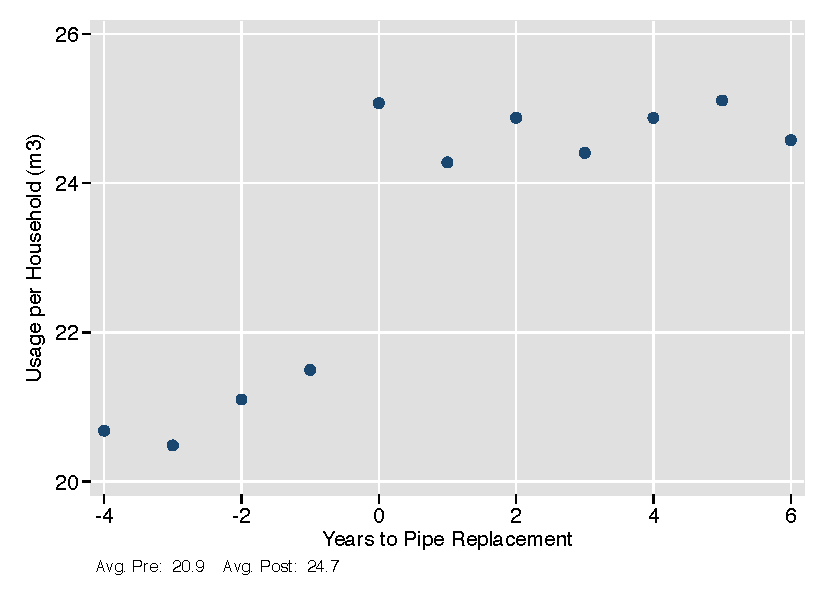
\includegraphics[scale=1]{tables/pipe_cons.pdf}
\end{center}
%%% add counts and average change in discussion
\end{figure}
% discuss dynamics!!! of figure!!

Mapping these increases in consumption into household welfare requires measuring how households trade off water usage and price.  Prices are determined by the government regulator who imposes an increasing tariff schedule according to monthly usage, which is standard among public utilities (\cite{hoque2013state}).  Despite steep increases in marginal price at specific levels of usage, households do not appear to be sensitive to these price changes because households are not observed adjusting their consumption strategically to avoid higher prices.\footnote{Appendix Figure~\ref{figure:tariffschedule} includes the average tariff schedule for users facing low and high prices.  Appendix Figure~\ref{figure:conshist} includes a histogram of usage per connection and finds little evidence of significant bunching at the tariff kink points at 10, 20, and 40 m3.}  The regulator also increases prices gradually over time to ensure that the company continues to cover operating costs.  Since households also gradually increase their average usage over this interval, it is unclear whether households are responsive to these price increases.\footnote{Appendix Figure~\ref{figure:pricetimeseries} plots average prices and usage per household over time.}

% [ RE-WRITE WITH NEW DEFINITION! ]
The empirical exercise analyzes an event-study where the same households are exposed to very different price levels over time.  The government regulator gives the water company discretion to assign households to a high-price tariff schedule if they have any business activity at their residence, which provides a novel source of price variation in the context of public utilities.  In the vast majority of cases, the high price tariff is applied to households that operate small food stands (or ``Sari-Sari'' stores).  For a household with average monthly usage, the high-price tariff results in an average price of 26.4PhP/m3 while the regular tariff results in an average price of 20.5PhP/m3.\footnote{Appendix~\ref{figure:tariffschedule} plots the tariff.}  The water company occasionally visits consumers and assigns consumers to the high-price tariff if business activity is observed at the residence.\footnote{In some cases, consumers request price decreases when they close their businesses.  These price-decrease events are not the focus of the analysis because consumers directly anticipate these events and may otherwise have adjusted their water usage accordingly.}  Table~\ref{table:pricechangestatistics} provides average characteristics of households that are observed with the regular price (in column (1)), that are observed with the high price (in column (2)), and that are observed increasing prices during the sample (in column (3)).  While the 724 households that experience price increases use more water than other households, they share similar demographic characteristics, which suggests that they may also share similar price-sensitivities.  

Figure~\ref{figure:usagepricechanges} plots average usage and marginal prices 4 years before and after households are first switched from the regular price to the high price.\footnote{In very few cases, households are later switched back to the regular price, and then switched again to the high price.}  Before the price change, average usage increases likely due to some households using additional water for their small-businesses.  The price change at month 0 is associated with a sharp drop in usage and increase in average prices that persist for at least 24 months.  These patterns indicate that household water usage is sensitive to large, discrete price changes over time.  


\begin{table}[h!] % PUT IN DEMOGRAPHICS PLEASE ?!?!?
\centering
\caption{Average Household Characteristics by Prices Charged}\label{table:pricechangestatistics}
\vspace{-2mm}
\begin{threeparttable}
\begin{tabular}{@{}l*{1}{KKK}@{}}
\toprule
  & Always Reg. Price & Always High Price  & Change Reg. to High Price \\
\midrule
Usage per Household (m3)& 19.95 & 20.17 & 23.42 \\
Household size & 4.98 & 4.74 & 4.99 \\
Employed members & 1.49 & 1.40 & 1.44 \\
High-skilled employment & 0.09 & 0.06 & 0.06 \\
Lives in duplex& 0.26 & 0.26 & 0.26 \\
Lives in single house& 0.50 & 0.59 & 0.54 \\
Other households sharing tap& 0.90 & 0.92 & 0.95 \\
\\[-.5em]
Households & 43,442 & 3,823 & 2,442 \\
\bottomrule
\end{tabular}
\begin{tablenotes}
\footnotesize
\item  Reg. refers to regular price.  

Pressure is 6 to midnight! Bill, Unpaid Balance, Payment, and Income are in PhP.  Measures exclude months where households remain disconnected through the end of the sample period.  Billing data include households for household-month observations.  Income data include households for household-month observations.  45 PhP = 1 USD \,\,
% See Appendix~\ref{appendix:sampleconstruction} for more details on the sample construction.
\end{tablenotes}
\end{threeparttable}
\end{table}

\begin{figure}
\begin{center}
\caption{Usage and Price Changes}\label{figure:usagepricechanges}
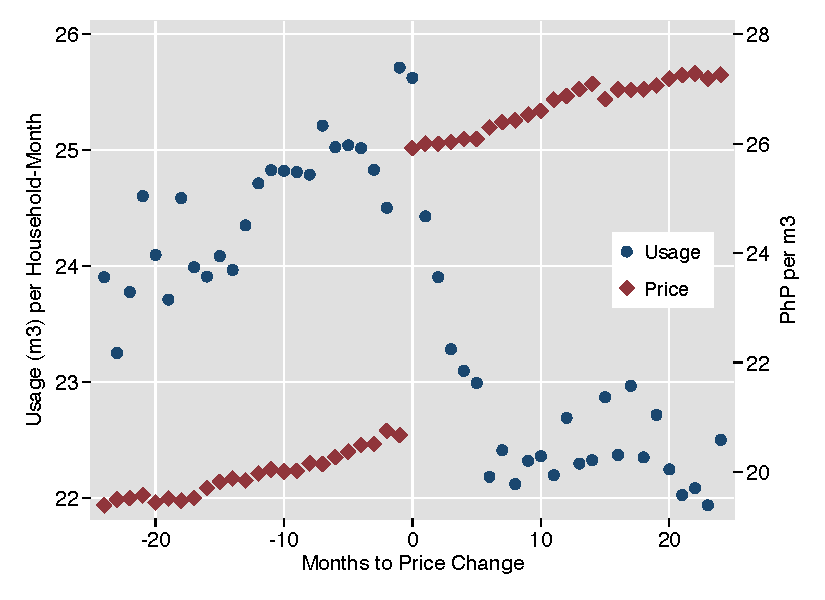
\includegraphics[scale=1]{tables/r_to_s_only_graph.pdf}
\end{center}
\end{figure}

\section{Model}

A simple model of household water demand connects changes in water usage and investments in water booster pumps to changes in household welfare as a result of pipe replacements.  In this model, households choose their monthly water usage as well as whether to use a booster pump to boost their water pressure.  

Each month, household utility takes the following form
\begin{align}
\label{eq:utility}
U\,=\,\frac{1}{\alpha} \, \Big[ \,  Q(B,R) \,  w  \, -\, \frac{1}{2}(w - \gamma)^2 \, \Big] \, + \, x 
\end{align}
where $w$ is water usage and $x$ represents a bundle of all other goods consumed by the household.  Water service quality given by the function, $Q(B,R)$, depends on booster pump use where $B$ equals 1 if the household chooses to use a booster pump (and zero otherwise) and as well as pipe replacements where $R$ equals 1 after pipe replacement (and zero otherwise).  $Q(B,R)$ is assumed to be differentiable in $R$.  Water service quality enters multiplicatively with water usage, which nests the assumption that each unit of water usage is affected equally and positively by water service quality.  This assumption also excludes the possibility that improved water service quality affects household utility in ways that are not directly proportional to household water usage such as by increasing housing values.  In this case, the approach would underestimate the welfare benefits of improved service quality.  $\alpha$ reflects price sensitivity, and $\gamma$ reflects the satiation amount of water usage.  This approach assumes that preferences for water are quasi-linear, which implies that water usage does not depend on household income [ Footnote to heterogeneity table ].  


% $\epsilon$ captures idiosyncratic monthly variation in satiation water usage such as changes in weather or in the number of household members using water.  $\epsilon$ is assumed to follow a normal distribution with zero mean and standard deviation $\sigma_{\epsilon}$.  
% The $\theta$ terms capture the household's preference for water service quality from booster pumps, pipe replacements, and the combination of the two.  
% For example, $\theta_3<0$ implies that booster pumps and pipe replacements are substitutable in producing water service quality.  

Households maximize utility subject to the following budget constraint
\begin{align}
\label{eq:bc}
p\,w \,+\, x \, +  B \, F \, = Y
\end{align}
where $p$ is the average price of water while the price of all other goods, $x$, is normalized to 1.  This approach includes the simplifying assumption that households respond to a single, average water price $p$ despite facing marginal prices that increase with monthly usage.  This assumption is consistent with descriptive evidence that households appear unresponsive to marginal prices.\footnote{Appendix Figure~\ref{figure:conshist} includes a histogram of usage per connection and finds little evidence of significant bunching at the tariff kink points at 10, 20, and 40 m3.}   $F$ is total cost of renting and using a booster pump each month.  This approach assumes that Manila has a competitive market for renting and selling booster pumps that is unaffected by improvements in piped water service quality.\footnote{This assumption is consistent with local service quality improvements and a city-wide market for booster pumps.}  $Y$ is monthly household income.  

% $\upsilon$ captures idiosyncratic monthly variation the booster pump cost such as changes in the electricity price or variation in installation costs. $\upsilon$ is assumed to follow a normal distribution that is assumed to be uncorrelated with $\epsilon$ and has zero mean and standard deviation $\sigma_{\upsilon}$.  

% as well as other research on public utility price responsiveness (\cite{ito2014consumers}, and the water ito paper?).  

Maximizing household utility in equation $(\ref{eq:utility})$ subject to the budget constraint in equation $(\ref{eq:bc})$ for a given choice of booster pump usage, $B$, yields the following expression for monthly water demand
\begin{align}
\label{eq:demand}
w(B) \, = \, \gamma \, - \, \alpha p +  Q(B,R)
\end{align}
Water demand depends linearly on the satiation preference, $\gamma$, price, and service quality.

Given optimal water demand, the indirect utility function at a given booster pump choice, $B$, is given by 
\begin{align}
V(B)\,=\,\frac{\alpha p^2}{2} - \gamma p + \frac{Q(B,R)^{2}}{2\alpha} - p Q(B,R) + \frac{\gamma Q(B,R)}{\alpha} + y - B F
\end{align}
The derivative of $V$ with respect to pipe replacements, $R$, reflects the change in consumer welfare associated with pipe replacements.  This derivative takes the following form after substituting terms for $w(B)$
\begin{align}
\label{eq:dvdr}
\frac{dV(B)}{dR}\,=\,\frac{w(B)}{\alpha} \frac{dQ}{dR} - F \frac{dB}{dR}
\end{align}
This expression summarizes the consumer welfare effects of pipe replacements in terms of (1) the marginal effect on service quality weighted by water usage and price sensitivity as well as (2) the marginal effect on booster pump usage weighted by the cost of booster pumps.  This approach assumes that welfare effects are proportional to usage, $w^{*}$, implying that service quality improvements affect all units of water usage.  Welfare effects are decreasing in price sensitivity, $\alpha$, which captures the intuition that households with many substitute water sources (ie. high $\alpha$) may benefit less from improvements in service quality.  According to this approach, welfare changes do not require measuring fixed preferences, $\gamma$, separately from levels of service quality, $Q(B,R)$.  Therefore, this approach is robust to different patterns of selection into booster pump use based on different levels of service quality or fixed preferences for water usage.  

% This feature is especially useful in the empirical setting where booster pump use is non-random across households.  
% The advantage of this approach is that welfare estimates do not require 
% Advantage in terms of unobservables, disadvantage in terms of counterfactuals...
% - Surplus is increasing in consumption (by assumption! given the multiplicative aspect)


\section{Empirical Strategy}

The empirical strategy estimates household price sensitivity as well as changes in water usage and booster pump use in response to pipe replacement projects. These estimated quantities inform the effect on consumer welfare of pipe replacement projects given by equation (\ref{eq:dvdr}).  Using an instrumental variables approach, the empirical strategy isolates price variation from connections being switched into high price tariffs.  The first stage equation takes the following form
\begin{align}
\label{eq:1ststage}
p_{it} &= \phi_1 \text{Post Pipe}_{tl}  +  \phi_2 \text{Post Price}_{it} +  \phi_3\text{Pre Trend}_{it} +\phi_4 \, \text{Post Trend}_{it} +  \phi_t  +  \phi_{il} + \epsilon_{itl} 
\end{align}
where $i$ indexes the water connection, $t$ indexes calendar month, and $l$ indexes small area.  $p_{it}$ is the average price per cubic meter of monthly water use.  $\text{Post Pipe}_{tl}$ is an indicator for months during and after January of the pipe replacement year.  $\text{Post Price}_{it}$ is an indicator for months after a connection is first switched into a high-price tariff.\footnote{In rare instances, connections may be switched into high-price tariffs more than once during the study period.  The instrumental variables design ensures that the estimation uses price variation only from the first price increase, which is more likely to be unexpected by households than later price increases.}  $\text{Post Price}_{it}$ is the instrumental variable that is excluded in the second stage.  To account for trends in water usage around the time of the price change, $\text{Pre Trend}_{it}$ counts the months leading up to the first price increase and takes a value of zero otherwise.  Likewise, $\text{Post Trend}_{it}$ counts months after the first price increase and takes a value of zero otherwise.  $\phi_t$ are calendar month fixed effects.  $\phi_{il}$ are connection fixed effects when the second stage has water usage as an outcome.  $\phi_{il}$ are small-area fixed effects when the second stage has booster pump use as an outcome because booster pump use is only observed in months where the connection survey was fielded.  

Given predicted prices from the first stage equation, the second stage equations take the following form
\begin{align}
w_{itl} &= \gamma_1  \text{Post Pipe}_{tl} + \gamma_2  \hat{p}_{it} + \gamma_3\text{Pre Trend}_{it} +\gamma_4\text{Post Trend}_{it} +    \gamma_t +  \gamma_i +  \varepsilon_{itl}  \label{eq:2ndstage1} \\
b_{itl} &= \beta_1  \text{Post Pipe}_{tl} + \beta_2  \hat{p}_{it} + \beta_3\text{Pre Trend}_{it} +\beta_4\text{Post Trend}_{it} +    \beta_t +  \beta_l +  \varepsilon_{itl} \label{eq:2ndstage2}
\end{align}
where $w_{itl}$ is water usage per household in cubic meters per month and $b_{itl}$ is an indicator for connection booster pump usage.  

The coefficients of interest for the impacts of pipe replacement are given by $\gamma_1$ and $\beta_1$ for water and booster pump use respectively.  After controlling for calendar month and connection fixed effects, these coefficients are identified from differential changes in outcomes for areas that experienced pipe replacements compared to areas that did not over the same interval.  These coefficients reflect the causal effect of pipe replacements under the assumption that no other factors changed at the same time that would otherwise affect the outcomes.  This assumption is supported by qualitative evidence that pipe replacements are often driven by hydrological, engineering concerns rather than strategic responses to changes in local water demand or other consumer characteristics.  Supporting this assumption, Figure~\ref{figure:pipecons} traces a sharp break in average usage at the year of pipe replacement with little evidence of strong trends before or after replacement projects.

The effects of prices on outcomes are given by $\gamma_2$ and $\beta_2$ for water and booster pump use respectively where $\hat{p}_{it}$ is the predicted price from the equation (\ref{eq:1ststage}).  The effects are identified from changes just before and after connections are switched to a high-price tariff after controlling for trends leading up to and after the tariff change.  The validity of this instrumental variables approach requires both that the tariff change produces a large impact on prices and that no other factors affect demand for water or booster pumps at the same time as the price change.  This approach assumes that while households may increase their water usage as they start small home businesses, households are unable to anticipate the exact timing of the price change so that any changes in water usage in the months just following the price change can be attributed to the higher prices.  Figure~\ref{figure:usagepricechanges} traces a smooth, increasing trend leading up to the price change.  Usage then drops abruptly at the same time as the price change, consistent with a surprise increase in prices.

The estimated coefficients directly inform the expression for welfare in equation (\ref{eq:dvdr}).  According to equation (\ref{eq:demand}), water quality linearly affects water demand.  Therefore, by capturing the effect of pipe replacements on water demand, $\gamma_1$ measures the total change in water quality from pipe replacements, $\frac{dQ}{dR}$.  $\beta_1$ measures the reduced form impact of pipe replacements on booster pump usage, $\frac{dB}{dR}$.  

The remaining term to be estimated in equation (\ref{eq:dvdr}) is the price sensitivity, $\alpha$.  $\gamma_2$ captures the reduced form effect of prices on water usage.  By taking the derivative of equation (\ref{eq:1ststage}) with respect to price, this effect can be expressed as a function of the price sensitivity as well as the effect of price on water quality through endogenous changes in booster pump use, according to the following equation
\begin{align*}
  \gamma_2 = \alpha +  \frac{dQ}{dB} \frac{dB}{dp}
\end{align*}
where $\frac{dQ}{dB}$ is the effect of booster pump use on water quality, which is unobserved.  $\frac{dB}{dp}$ is the effect of prices on booster pump use, which is estimated by $\beta_2$.  If $\frac{dB}{dp}$ is zero, then the expression reduces to $\gamma_2=\alpha$.  Although the booster pump decision is not explicitly modeled, $\frac{dB}{dp}$ may be zero or close to zero when booster pump use is primarily driven by other factors besides the price of water.  For example, booster pumps may be a perfect substitute for water quality such that all households below a certain water quality level choose to use booster pumps while all households above this level do not use booster pumps.  In this example, the booster pump decision is orthogonal to water prices.  

Given fixed effects the are identified from 

When the outcome is monthly water usage, the estimating equation maps directly onto the equation for optimal household usage given by equation ($\ref{eq:demand}$).  $\beta_1$ captures the effect of pipe replacement on service quality, $\frac{dQ}{dR}$.  Likewise, $\beta_2$ captures the negative of household price sensitivity, $\alpha$.  Remaining fixed preferences for water and levels of service quality are absorbed in household and month fixed effects, $\lambda_i$ and $\theta_t$.  These fixed effects ensure that the effect of pipe replacements is identified from variation in water usage for the same household before and after pipes are fixed while accounting for any temporal usage patterns common to all households.  Likewise, price sensitivity is estimated from variation in price for the same household switching between regular and high prices.  Calendar month fixed effects absorb price variation affecting all households equally over time as the company updates water tariffs.  

When the outcome is booster pump use, the estimating equation captures the effect of pipe replacements on booster pump use.  This approach assumes that demand for booster pumps can be linearly approximated by the estimating equation such that $\beta_1$ reflects $\frac{dB}{dR}$.  Since booster pump use is a binary outcome, this approach represents a linear probability model.  Time fixed effects account for variation in booster pump usage over time common to all households while household fixed effects account for differences in booster pump use across households.  $\beta_1$ reflects the effect of pipe replacements on booster pump use under the assumption that no other factors independently affect booster pump use at the same time.  One concern may be that the prices for booster pumps change in response to pipe replacement projects.  Pipe replacements occur in small geographic areas while markets for booster pumps are likely to cover much wider areas.\footnote{Online markets span the entire city.}  Therefore, individual pipe replacement projects are unlikely to influence prices for booster pumps.

% \begin{align}
% \label{eq:1ststage}
% p_{it} &= \phi_1 \text{Post Pipe Rep}_{tl}  +  \phi_2 \text{Post Price Inc}_{it} +  \phi_3\, t\text{ Post Price Inc}_{it} +\phi_4 \,t \,\text{Pre Price Inc}_{it} +  \phi_t  +  \phi_i + \epsilon_{itl} 
% \end{align}
% \begin{align}
% \label{eq:1ststage}
% p_{it} &= \phi_1 \mathbbm{1} \{t\geq \text{Pipe Rep}_{tl}  \} +  \phi_2 \mathbbm{1} \{t\geq \text{High Price}_{tl}  \} +  \phi_3\, t \, \{t\geq \text{High Price}_{tl}  \} +\phi_4 \,t \,\{t< \text{High Price}_{tl}  \} +  \phi_t  +  \phi_i + \epsilon_{itl} 
% \end{align}
% The estimating equation takes the following form
% \begin{align}
% \label{eq:esteq}
% y_{itl} \,=\, \beta_1 \, \text{After Pipe Replacement}_{tl} \,+\, \beta_2 \, p_{it} \, + \, \theta_t \, + \, \lambda_i \, + \epsilon_{itl}
% \end{align}
% where the outcome, $y_{itl}$, is either monthly water usage or booster pump use.  Outcomes are measured for household, $i$, in small area, $l$, at calendar month, $t$. After Pipe $\text{Replacement}_{tl} $ takes a value of one for months after pipe replacement and zero otherwise.  Since the data identify only the year that pipes were replaced, all months from the replacement year onwards are considered after pipe replacement. $p_{it}$ measures the average price faced by each household in each month. $\theta_t$ includes calendar month fixed effects while $\lambda_i$ includes household fixed effects.


% This approach also assumes that booster pumps do not impose substantial negative externalities on local water service quality.  A recent engineering literature has raised the possibility that booster pumps interfere with water flow in pipe mainlines, reducing pressure along the entire pipe (\cite{taylor2014reducing}).  However, this problem may not be as salient in the context of Manila.  The water company has not raised booster pumps as a policy problem in any of their internal documents.\footnote{Booster pumps are sometimes mentioned in water company investigations of consumer complaints as an explanation for household water pressure and never as problem to be addressed.}  Moreover, externalities would predict large water usage gaps between those with and without booster pumps in the same neighborhood.  By contrast, Table~\ref{table:usageregs} finds a similar association of booster pump use and water usage with and without small-area fixed effects.   % Taken together, the empirical evidence is supportive of the relatively strong assumptions necessary to identify booster pump preferences.


\section{Results}

Table~\ref{table:mainregs} includes results of the effect of price and pipe replacements.  Column (1) provides results on household water use finding an increase of 1.79 m3 per household per month after pipe replacement.  The estimate is statistically significant at the 1\% and economically large representing an 8\% increase in average usage.  The estimated increase is smaller than the descriptive increase in Figure~\ref{figure:pipecons} likely because the regression approach controls for increasing trends in water use over the sample period.  

Column (1) also provides an estimated price sensitivity of 0.17, which is statistically significant at the 1\% level.  Given an average price of 21.5 PhP/m3, this estimate also implies a price elasticity of 0.17.  This elasticity estimate is on the lower end of similar studies in the developing world, which find elasticities ranging from 0.01 to 0.98.\footnote{See \cite{szabo2015value}, \cite{diakite2009proposal}, and \cite{strand2005water}.}  

Column (2) finds that pipe replacement projects are associated with a 20\% decrease in booster pump use, which is statistically significant at the 5\% level.  This decline is smaller than the descriptive decline in Table~\ref{table:descriptives} likely since the regression approach accounts for decreasing booster pump use over the sample period.

% While previous studies largely focus on cities in low-income countries (\cite{diakite2009proposal} ) or low-income neighborhoods within larger cities, this estimate  which may explain 

% dQ/Q / dP/P  =  (.17/22.14) /  (1/21.5)
% This estimate is in range of the 0.98 estimate from \cite{szabo2015value} as well as similar studies in the developing world that find elasticities between 0.01 and 0.81 (\cite{diakite2009proposal}, \cite{strand2005water}). 

\begin{table}[h!] 
\centering
\caption{Household Water and Booster Pump Use Estimates}\label{table:mainregs}
\vspace{-2mm} 
\begin{threeparttable}
\begin{tabular}{@{}l*{1}{CC}@{}}
\toprule
  & (1)       & (2)              \\
  & Water Use & Booster Pump Use \\
\midrule
After Pipe Replacement&        1.89\textsuperscript{a}&       -0.20\textsuperscript{b}\\
                    &      (0.13)                   &      (0.08)                   \\
Avg. Price (PhP)    &       -0.15\textsuperscript{a}&       -0.00                   \\
                    &      (0.05)                   &      (0.02)                   \\
Mean                &       19.83                   &        0.16                   \\
$\text{R}^{2}$      &       0.554                   &       0.942                   \\
N                   &   4,004,448                   &      49,319                   \\
Dataset             &Billing Panel                   &Household Survey                   \\

\bottomrule
\end{tabular}
\begin{tablenotes}
\footnotesize
\item Weighting, discussion of different samples, clustering, controls (especially rate classes).  This table predicts usage per household with pipe replacement and price with different fixed effects.  
\end{tablenotes}
\end{threeparttable}
\end{table}




\begin{table}[h!] 
\centering
\caption{Change in Consumer Surplus}\label{table:mainregs}
\vspace{-2mm}
\begin{threeparttable}
\begin{tabular}{@{}l*{1}{CCC}@{}}
\toprule
            & Service Quality              & Booster Pump Use & Total             \\
\midrule
Expression  & $\frac{w^{*}}{\alpha} \frac{dQ}{dR}$ &   $- F \frac{dB^{*}}{dR}$  & $\frac{dV}{dR}$ \\[1em]
Estimates   &   249.7 & 97.1 & 346.8 \\
            &  (109.6) & (16.8) & (103.7)  \\
% Evaluated Estimates \\
\bottomrule
\end{tabular}
\begin{tablenotes}
\footnotesize
\item Weighting, discussion of different samples, clustering, controls (especially rate classes).  This table predicts usage per household with pipe replacement and price with different fixed effects.  
\end{tablenotes}
\end{threeparttable}
\end{table}







Fixed costs:

On average, pipe replacement projects replace 25.3 km of pipes at a cost of 166 million PhP.  The average cost per pipe length is 9 million PhP per kilometer.  Since around 0.73 km of pipes are replaced per small area, total project costs per small area are around 6.6 million PhP.  With 275 connections per small area, project costs average 24,000 PhP per connection.   

6.6 million PhP/(275*1.41)


New Revenues:

Residential connections are billed 68 PhP more per month while commercial connections are billed 145 PhP more per month.  Given that 94\% of connections are residential and 6\% of commercial, the total billing increase is around 73 PhP per month per connection.  

Decrease in Marginal Costs:

After pipe-replacement, usage per connection decreases by 21 m3 per month.  Given marginal costs of 5 PhP per m3, then this decrease implies a cost reduction of 105 PhP per month.  


((73 )*12)/24000
((400)*12)/24000
((73 + 105 + 80)*12)/24000



\begin{table}[h!] 
\centering
\caption{Total Water Supplied and Billed Estimates}\label{table:nrwregs}
\vspace{-2mm}
\begin{threeparttable}
\begin{tabular}{@{}l*{1}{CCCCC}@{}}
\toprule
  & (1)   & (2)   & (3) \\
  & Volume Billed  & Volume Supplied & \% Non-Revenue Water \\
\midrule
After Pipe Replacement&        1.64                   &      -21.27\textsuperscript{a}&       -0.20\textsuperscript{a}\\
                    &      (1.90)                   &      (6.54)                   &      (0.03)                   \\
Mean                &       26.54                   &       39.53                   &        0.28                   \\
$\text{R}^{2}$      &       0.892                   &       0.798                   &       0.595                   \\
N                   &      67,827                   &      67,827                   &      67,824                   \\

\bottomrule
\end{tabular}
\begin{tablenotes}
\footnotesize
\item Say it includes both fixed effects (Describe fixed effects...) .  Weighting, discussion of different samples, clustering, controls (especially rate classes).  This table predicts usage per household with pipe replacement and price with different fixed effects.   \regtext 45 PhP = 1 USD \,\,
\end{tablenotes}
\end{threeparttable}
\end{table}






\begin{table}[h!] 
\centering
\caption{Usage per Connection Regression Estimates}\label{table:profitregs}
\vspace{-2mm}
\begin{threeparttable}
\begin{tabular}{@{}l*{1}{cccc}@{}}
\toprule
  & (1) & (2) & (3) & (4)  \\
  & Usage (m3) & Bill (PhP) & Usage (m3) & Bill (PhP) \\
\midrule
After Pipe Replacement&        2.56\textsuperscript{a}&       72.90\textsuperscript{a}&        3.21\textsuperscript{a}&      144.76\textsuperscript{a}\\
                    &      (0.17)                   &      (6.04)                   &      (0.33)                   &     (26.43)                   \\
Mean                &       27.96                   &      699.18                   &       49.98                   &    3,253.21                   \\
Connection Type     & Residential                   & Residential                   &  Commercial                   &  Commercial                   \\
$\text{R}^{2}$      &       0.568                   &       0.567                   &       0.683                   &       0.718                   \\
N                   &   4,012,392                   &   4,010,876                   &   4,557,094                   &   4,550,439                   \\

\bottomrule
\end{tabular}
\begin{tablenotes}
\footnotesize
\item Weighting, discussion of different samples, clustering, controls (especially rate classes).  This table predicts usage per household with pipe replacement and price with different fixed effects.   \regtext 45 PhP = 1 USD \,\,
\end{tablenotes}
\end{threeparttable}
\end{table}



%%% leave out booster pumps?
\section{Counterfactuals}

% We're focusing on a part of the natural monopoly where the costs are easy to measure (you replace pipes), but the benefits are less well understood.  Different from the standard Laffont and Tirole model; closer to the Spence model which is a real contribution!  (luckily high cost areas also have high benefit)

% Set aside all other aspects of regulation to focus on quality!  Usually, capital is thought of as an input to deliver a certain quantity of the product.  Here we're focusing on a particular 

The following counterfactuals identify the welfare effects of optimal pipe replacements under five different information environments.  The counterfactuals focus on the role of pipe replacements by holding fixed other aspects of water utility regulation.  The full population of Manila is assumed to remain connected to service indefinitely.  The water tariff is assumed to be determined independently of pipe replacements and to exactly cover all costs of water production (except pipe replacements).  Unless otherwise specified, any cost savings or cost overruns as a result of the pipe replacements are assumed to be passed on to consumers in the form of fixed rebates or charges, which do not affect consumers' marginal incentives to consume water.  Pipe replacements are assumed to be independent of operating costs such as labor or maintenance expenditures.

% The \textit{full-information} counterfactual provides an optimal benchmark where the regulator chooses when to replace pipes to maximize total welfare given full information on demand and costs.  In the \textit{regular-replacement} counterfactual, the regulator simply replaces all pipes at a fixed interval.  In the \textit{quality-standards} counterfactual, the regulator establishes a minimum water pressure threshold and replaces pipes when pressure falls below the threshold.  In the \textit{cost-recovery} counterfactual, the regulator schedules replacements to balance savings from lower pumping costs against upfront costs of the pipe replacements.  In the \textit{firm-level} counterfactual, the regulator lets the firm decide when to replace pipes under the assumption that the firm has full demand and cost information.

% - hold price fixed!
% - decide replacements independently for each area
% - 

% - Not permitted expenses, similar to a price-cap [that's fair] (under invest)
% - Rate of return (allow for overlapping loans...?) --> no, don't ; make the point that the firm will want to replace pipes as soon as loans come due because the projects generate more than enough revenue to meet reasonable rates of return.  

% - permitted expenses or not? hard to know..
% - rate of return when we don't know the production function; 
% - high power --> redistribute little but keep costs down
% - low power --> redistribute a lot but high costs
% --- where are we?

% --> low power: all the surplus goes to consumers, but decisions are based on limited information
% --> high power: firm can get the surplus, but decisions are based on detailed consumer information; provides a strong incentive for the firm to figure out exactly the benefits of the investments
%%% in practice, it's somewhere between
%%% note that with the high power incentive, the prices are high, and the wedges get smaller if the prices are lower!
%%% footnote explaining distinction with standard high versus low-powered incentives.

% Since these projects generate streams of revenues in excess of their costs, then rate-of-return regulation would likely lead firms to very frequently replace pipes.\footnote{We do not explicitly model rate of return regulation here because the constraint would depend on whether the company could take out multiple loans, and the cost of capital for those loans.}



The \textit{full-information} counterfactual simulates how often a regulator would optimally replace pipes in order to maximize welfare under full information.  For each section of the service area, the regulator maximizes present-discounted consumer welfare indefinitely given by the following expression
% doublecheck the tau's and t's
\begin{align*}
max_{R_t\in\{0,1\}} \,\, &\sum_{\tau = t}^{\infty} (1+\delta)^{t-\tau} [CS(k_{t}) + V(k_{t})]  \\
V(k_{t}) &= W(k_{t}) - E(k_{t}) - L(k_{t})\\ 
k_{t+1} &=  (1 + k_t) \, (1-R_t \mathbbm{1} \{ k_{t}> l\}) \\
L(k_t) &= \frac{r(1+r)^{l} }{(1+r)^{l} -1 }\overline{L} \, \mathbbm{1} \{ k_{t}\leq l \}
\end{align*}
where $t$ indexes month, $\delta(>0)$ is the discount factor, and $k_t$ is the age of the pipes.  $CS(k_{t})$ is the consumer surplus from pipe replacements as defined in equation (ref!), which is assumed to be decreasing in pipe age.  $V(k_t)$ is the net revenue from pipe replacements, which depends on revenue from (increased) water sales, $W(k_{t})$, costs of water leakage, $E(k_{t})$, and payments on any loans to fund pipe replacements, $L(k_t)$.  $V(k_t)$ is passed on to consumers as a fixed rebate or charge (ie. by adjusting the monthly service charge).  Due to pipe deterioration, consumer surplus and water revenue are both assumed to be decreasing in pipe age while water leakage is assumed to increase with pipe page.  

Each month, the regulator chooses whether to replace pipes ($R_t = 1$) or not ($R_t = 0$).  Replacing pipes sets the pipe age, $k_t$, back to zero and is only possible if the regulator has paid off any debt from a previous pipe replacement where $l$ indexes the duration of the debt.  The regulator is assumed to fund a pipe replacement with a loan of total size, $\overline{L}$, at monthly interest rate, $r$, over duration, $l$.  The expression for $L(k_t)$ calculates the size of the monthly loan payments.  In this framework, the optimal schedule of pipe replacements balances net revenue against consumer surplus from new pipes.


% While in practice, regulators may adjust both marginal prices and fixed monthly service charges, the model focuses only on fixed monthly service charges  
% The model implicitly assumes that the regulator is able to implement fixed transfers to and from consumers without distorting their water consumption.  For example, the regulator may offer all consumers fixed rebates in months with budget surpluses and higher fixed water charges in months with budget deficits.  
% Allowing negative net revenues in the model provides an approximation for this scheduling optimization.

% While the model does not explicitly capture scheduling optimization, it 
% This framework also holds the water tariff fixed.  


In the \textit{regular-replacement} counterfactual, the regulator only observes the age of the pipes and chooses to replace pipes as soon as they reach a certain age, $\overline{K}$.  In the \textit{quality-standards} counterfactual, the regulator also observes the water pressure reaching consumers, $P(k_t)$.  The regulator then chooses to replace pipes once the water pressure falls below a certain threshold, $\overline{P}$.  In the \textit{cost-recovery} counterfactual, the regulator does not observe water pressure, but instead observes leakage costs.  The regulator then replaces pipes to minimize leakage costs, $E(k_{t})$ and pipe replacement costs, $L(k_{t})$.  

% The marginal price is enough to cover the other fixed costs, and the firm gets to keep the leftovers!

In the \textit{firm-level} counterfactual, the regulated firm is assumed to be fully aware of not only leakage costs, $E(k_t)$, but also revenue from water sales as result of pipe replacements, $W(k_t)$.  To incentivize the firm to act on this information, the regulator allows the firm to enjoy the net revenues from pipe replacements, $V(k_t)$.  The firm then chooses replacement rates to maximize, $V(k_t)$.  In this case, consumer surplus, $CS(k_t)$ is equal to consumer welfare because consumers no longer receive transfers equal to net revenues.  This arrangement is equivalent to ``price-cap'' regulation where the regulator sets a maximum price and firm is able to enjoy profits at prices up to the maximum while incurring investment costs.\footnote{See \cite{joskow2007regulation}.}




Specify, exactly what is allowed to vary across places and what isn't!

The simulations assume an annual discount factor of $\delta$=4\% and an annual interest rate of $r=5\%$, which is consistent with loans covering recent water investments.  


Costs, $L_()$, are measured... 


% and the regulator allows the firm to maximize producer surplus, $PS(k) - L(k_{t})$.

% Total welfare versus producer/consumer divide?


% Mermelstein et al. (2012) for dynamic merger analysis
%%% in some months, it may be negative..


% Discuss the empirical set up!  Discuss the limitations in the empirical set-up. Roughly correspond to natural divisions of the service area.

Consumer surplus and producer surplus are assumed to linearly decline in pipe age, $k_t$.  This assumption is consistent with civil engineering research documenting a roughly linear relationship between pipe failure and age.\footnote{See \cite{ward2017deterioration}, \cite{kleiner2001comprehensive}, and \cite{aydogdu2015estimation}.}  




Since the majority of pipes are replaced 

Appendix on decom.




Results are discussed below in Table [x].

 then the regulator maximization problem has an interior solution where the regulator choses whether to .  In practice, simulations solve the maximization problem recursively using 

% This approach abstracts away from many other features (price, independent decisions, maintenance, expectations about the future)

% where $t$ indexes month, $\delta>0$ is the discount factor, and $k_t$ is the age of the pipes.  $CS(k_{t})$ is consumer surplus and $PS(k_{t})$ is producer surplus, which are both assumed to be decreasing in pipe age as pipes deteriorate.  $L(k_{t})$ is the payment on the loans needed to fund upfront pipe replacements.  Each month, the regulator chooses whether to replace pipes ($R_t = 1$) or not ($R_t = 0$).  Replacing pipes sets the pipe age, $k_t$, back to zero and is only possible if the regulator has paid off any debt from a previous pipe replacement where $l$ indexes the duration of the debt.  The regulator is assumed to fund pipe replacements with a loan of total size, $\overline{L}$, at monthly interest rate, $r$, over duration, $l$.  The expression for $L(k_t)$ calculates the monthly loan payment for the duration of the loan.  In this framework, the optimal schedule of pipe replacements balances the (decreasing) consumer and producer surplus from new pipes against the upfront cost of replacing pipes.  

% In the \textit{regular-replacement} counterfactual, the regulator is uninformed about consumer and producer surplus.  Instead, the regulator only knows the age of the pipes and chooses to replace pipes as soon as they reach a certain age, $\overline{K}$.  In the \textit{quality-standards} counterfactual, the regulator observes not only the age of the pipes, but also the water pressure reaching consumers, $P(k_t)$.  The regulator then chooses to replace pipes once the water pressure falls below a certain threshold, $\overline{P}$.  In the \textit{cost-recovery} counterfactual, the regulator does not observe water pressure, but instead observes the part of producer surplus attributable to leakage costs, $E(k_t)$.  The regulator then replaces pipes to minimize leakage costs and pipe replacement costs.  

% In the \textit{firm-level} counterfactual, the regulated firm is assumed to be fully aware of producer surplus, $PS(k)$, and the regulator allows the firm to maximize producer surplus, $PS(k) - L(k_{t})$.

% Total welfare versus producer/consumer divide?


% k_{t+1} &= \begin{cases}
% k_t + 1 &\text{ if } R_t=0 \\
% 0 &\text{ if } R_t=1 \text{ and } k_{t}> l
% \end{cases}\\
% \begin{align*}
% L(k_t) = \begin{cases}
% \overline{L}\frac{r(1+r)^{l} }{(1+r)^{l} -1 } &\text{ if } k_{t}\leq l \\
% 0 &\text{ if } k_{t}> l
% \end{cases}
% \end{align*}
% d = (((1+r)^(12*loan_term))-1)/(r*(1+r)^(12*loan_term));
% F  = total_loan/d;




The fourth counterfactual imagines an uninformed regulator and a fully informed firm where the firm decides when to replace pipes.  The regulator does not adjust prices to compensate the firm for pipe replacements, which leaves the firm to maximize its own surplus from replacing pipes.\footnote{Strong incentive to reduce costs: This may occur when the regulator can't credibly commit to price increases or when the firm has a strong incentive to inflate costs which the regulator cannot verify.}




according to advice from water engineers who measure costs of replacements as well as pumping cost savings.  The regulator then replaces pipes to optimize upfront replacement costs against marginal savings in pumping costs.

without knowing the replacement costs or how replacements would affect water demand.  However, the regulator is able to measure water pressure either through consumer surveys, consumer complaints, or pressure gauges.  The regulator then establishes a minimum pressure threshold and replaces pipes when the pressure drops below the threshold.


Section Welfare:
	- Welfare benefits with 10 yr 5\% loans (assume discount rates) or 50 yr 5\% loan?
	- Welfare benefits with cash
	- Are households willing to pay for pipe improvements?

	- How do welfare estimates compare to traditional estimates from health measures?

Robustness:
	- Use nearest pipe replacement definition (selection into meter identification)



% - Discusses use of booster pumps in Clean Water Act 2004:  https://www.manilatimes.net/2018/11/04/legal-advice/dearpao/use-of-booster-pumps/461829/  http://r12.emb.gov.ph/ra-9275-the-philippine-clean-water-act/
% - https://idl-bnc-idrc.dspacedirect.org/bitstream/handle/10625/14878/108376.pdf?sequence=5
% - illegal booster pumps :  Consequence of El Niño 1997-98 on Manila water resources: new perspectives in water shortage management
% - seizing booster pumps : https://timesofindia.indiatimes.com/city/navi-mumbai/booster-pumps-used-by-some-socs-leading-to-water-crunch/articleshow/68856763.cms , https://timesofindia.indiatimes.com/city/nagpur/215-booster-pumps-seized/articleshow/69804589.cms




 % If households were sensitive to price increases at specific consumption levels, then households would be expected to frequently consume just below these levels.  However, Appendix Figure plots the frequency 






% The welfare benefits of fixing water pipes depends on which dimensions of service quality are improved by pipe replacement.  Table~\ref{table:descriptives} compares average household survey responses before and after pipe replacement.

% Allow services that they couldn't before

% Before pipe replacement, households experience weak water pressure and low water quality.  30\% of households report generally having no water pressure from 6 pm to 12 am in the absence of an extra household pump to boost water pressure.  23\% of households report that their piped water generally has foreign bodies.

% To compensate for low piped water quality, many households invest in private water booster pumps, storage drums, water filters, and purchases of non-piped water.  

% Both pressure and water quality improve substantially following pipe replacement.  The shares of households reporting no water pressure, water discoloration, foreign bodies, and unusual tastes/smells all drop to below 6\%.  

% - Quality complements more consumption
% - Water quality implies that consume the same, just enjoy it wayyy more
% 	- maybe need to clean things longer
% 	- maybe clean things the same but get way more utility

% - Pressure implies that quantity is positively linked to quality!
% 	- has the same feature?
% 	- use the same water, just less time...
% 	- costly to push for that extra water..... from a time perspective
% 		- Natural to think of relieving the pressure as leading to greater consumption!




	% Table: 
	% 	(A) What does pipe fixing mean?
	% 		- Quality, Hours, Flow

	% 	(B) How do households change their investments?

	% 	(C) How do households use their water?

	% 	(D) Household demographics including sharing
	% 		* N 
	% 	(E) Household consumption/payments/disconnection/standard deviation! (from billing data N)
	% 		* N




%%%% PIPE AGE %%%  possibly lower quality as well
% http://www.mayniladwater.com.ph/news-article.php?id=656
% West Zone concessionaire Maynilad Water Services, Inc. (Maynilad) replaced a total of 196 kilometers of old pipes in 2016, bringing the total length of pipes replaced within its concession area to 1,709 kilometers—about the same distance from Manila to Hanoi, Vietnam—since the company’s re-privatization in 2007.
% Maynilad invested ₱1.85 billion for its pipe replacement projects in 2016 alone. The old pipelines rehabilitated last year were located mostly in Quezon City, Manila and Bacoor City, where “pipe age” ranged from 30 to 40 years.
% http://www.mayniladwater.com.ph/news-article.php?id=366
% Maynilad spends 77M to replace 24km pipes in Malabon
% July 03, 2013

% West Zone concessionaire Maynilad Water Services, Inc. (Maynilad) is replacing 23.6 kilometers of secondary and tertiary pipes in Malabon City to improve services to more than 12,800 households in the area. The water company is spending some P77 million to replace the 30-year old pipes by the 3rd quarter of 2013.

% % doesn't dramatically change substitution to other sources!

% Reference Hanoi for how households may care about water use
% 	- percentages

% --- Water pump depreciation!?

% Figure consumption graph for effect dynamics (appendix with all other effect dynamics)

% Figures no bunching; small changes over time
% 	- Cite a bunch of other papers here... novel identification....

% Figures price variation and selection into switchers...
% 	- examine robustness to alternative alpha definitions...


\section{Appendix}







% \begin{table}[h!] 
% \centering
% \caption{Booster Pump Use Regression Estimates}\label{table:boosterregs}
% \vspace{-2mm}
% \begin{threeparttable}
% \begin{tabular}{@{}l*{1}{ccc}@{}}
% \toprule
%   & (1) & (2) & (3)  \\
% \midrule
% After Pipe Replacement&      -0.101\textsuperscript{a}&      -0.101\textsuperscript{a}&      -0.091\textsuperscript{a}\\
                    &     (0.011)                   &     (0.011)                   &     (0.008)                   \\
Pipe Replacement Area&       0.212\textsuperscript{a}&       0.212\textsuperscript{a}&                               \\
                    &     (0.015)                   &     (0.015)                   &                               \\
Avg. Price (PhP)    &                               &       0.001                   &       0.000                   \\
                    &                               &     (0.002)                   &     (0.002)                   \\
Ever High Price     &                               &      -0.012                   &       0.003                   \\
                    &                               &     (0.011)                   &     (0.010)                   \\
Ever Change Price   &                               &      -0.015                   &      -0.012                   \\
                    &                               &     (0.010)                   &     (0.010)                   \\
Household Size      &                               &      -0.001                   &       0.000                   \\
                    &                               &     (0.001)                   &     (0.001)                   \\
Employed Household Members&                               &       0.012\textsuperscript{a}&       0.010\textsuperscript{a}\\
                    &                               &     (0.002)                   &     (0.001)                   \\
High Skilled Employment&                               &       0.086\textsuperscript{a}&       0.081\textsuperscript{a}\\
                    &                               &     (0.007)                   &     (0.006)                   \\
Mean                &        0.15                   &        0.15                   &        0.15                   \\
Calendar Month FE   &  \checkmark                   &  \checkmark                   &  \checkmark                   \\
Small-Area FE       &                               &                               &  \checkmark                   \\
$\text{R}^{2}$      &       0.069                   &       0.076                   &       0.291                   \\
N                   &   2,379,456                   &   2,379,456                   &   2,379,456                   \\

% \bottomrule
% \end{tabular}
% \begin{tablenotes}
% \footnotesize
% \item This table predicts household booster pump use with pipe replacement including demographic controls and small-area fixed effects.   \regtext 45 PhP = 1 USD \,\,
% \end{tablenotes}
% \end{threeparttable}
% \end{table}







\begin{figure}
\begin{center}
\caption{Price Time-Series}\label{figure:pricetimeseries}
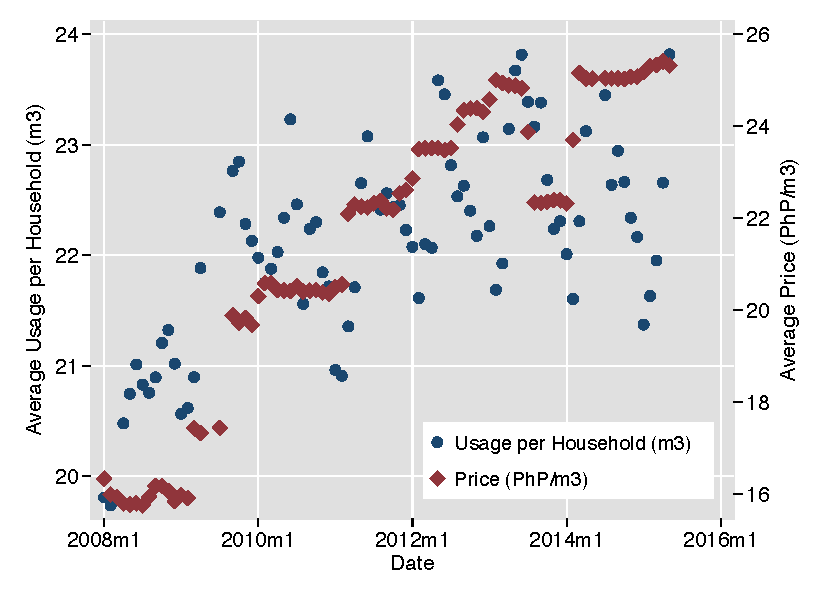
\includegraphics[scale=1]{tables/price_time_series.pdf}
\end{center}
\end{figure}


\begin{figure}
\begin{center}
\caption{Tariff Schedule}\label{figure:tariffschedule}
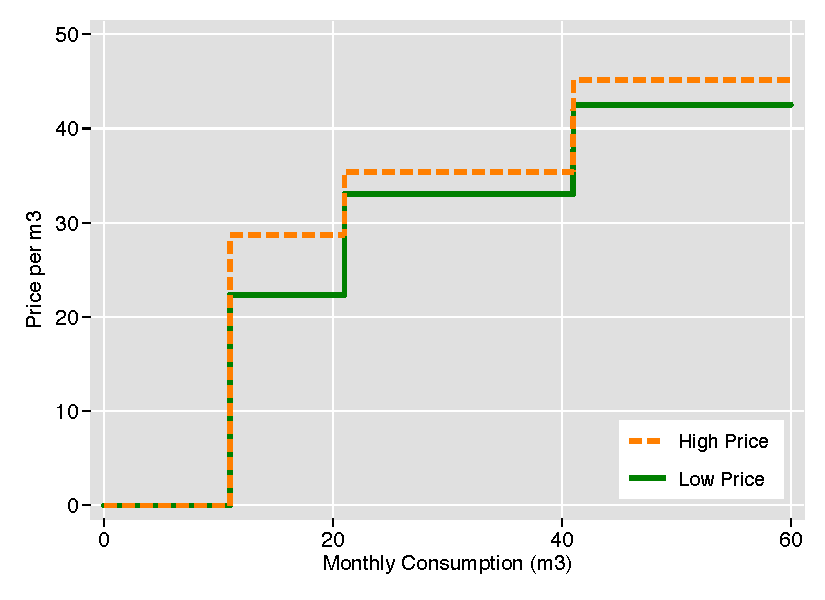
\includegraphics[scale=1]{tables/rs_prices.pdf}
\end{center}
\end{figure}

\begin{figure}
\begin{center}
\caption{Usage Histogram}\label{figure:conshist}
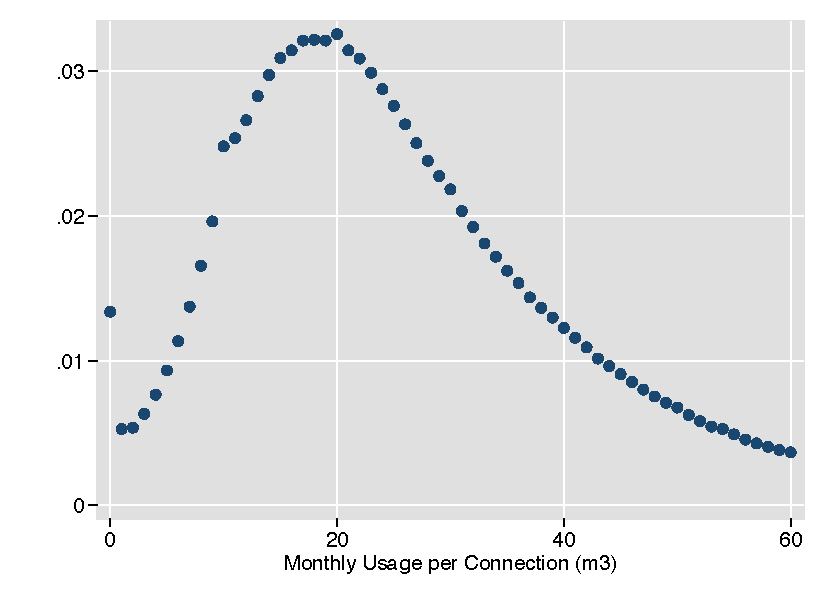
\includegraphics[scale=1]{tables/cons_histogram.pdf}
\end{center}
\end{figure}



\begin{table}[h!] 
\centering
\caption{Water and Booster Pump Use per Household Estimates}\label{table:mainregshet}
\vspace{-2mm}
\begin{threeparttable}
\begin{tabular}{@{}l*{1}{CCCC}@{}}
\toprule
  & (1)       & (2)  & (3) & (4)            \\
  & Water Use & Water Use  & Booster Pump Use & Booster Pump Use \\
\midrule
Post                &        1.57\textsuperscript{a}&        1.69\textsuperscript{b}&       -0.21\textsuperscript{a}&       -0.21\textsuperscript{b}\\
                    &      (0.28)                   &      (0.80)                   &      (0.02)                   &      (0.09)                   \\
Avg. Price (PhP)    &       -0.15\textsuperscript{a}&       -0.11                   &        0.00                   &        0.00                   \\
                    &      (0.05)                   &      (0.16)                   &      (0.00)                   &      (0.00)                   \\
Post $\times$ Household Size&       -0.00                   &                               &       -0.00                   &                               \\
                    &      (0.05)                   &                               &      (0.00)                   &                               \\
Post $\times$ Employed Household Members&       -0.15\textsuperscript{c}&                               &        0.01                   &                               \\
                    &      (0.08)                   &                               &      (0.00)                   &                               \\
Post $\times$ High Skilled Employment&       -1.10\textsuperscript{a}&                               &       -0.01                   &                               \\
                    &      (0.28)                   &                               &      (0.02)                   &                               \\
Post $\times$ Subdivided House/Duplex&        0.59\textsuperscript{b}&                               &        0.01                   &                               \\
                    &      (0.25)                   &                               &      (0.01)                   &                               \\
Post $\times$ Freestanding House&        1.04\textsuperscript{a}&                               &        0.01                   &                               \\
                    &      (0.22)                   &                               &      (0.01)                   &                               \\
Post $\times$ Monthly Income (10,000 PhPs)&                               &       -0.38                   &                               &        0.05                   \\
                    &                               &      (0.43)                   &                               &      (0.05)                   \\
Household Size      &        1.68\textsuperscript{a}&                               &        0.00                   &                               \\
                    &      (0.09)                   &                               &      (0.00)                   &                               \\
Employed Household Members&        0.20                   &                               &        0.00\textsuperscript{b}&                               \\
                    &      (0.13)                   &                               &      (0.00)                   &                               \\
High Skilled Employment&        0.00                   &                               &        0.07\textsuperscript{a}&                               \\
                    &      (0.48)                   &                               &      (0.01)                   &                               \\
Subdivided House/Duplex&       -1.31\textsuperscript{a}&                               &       -0.05\textsuperscript{a}&                               \\
                    &      (0.40)                   &                               &      (0.01)                   &                               \\
Freestanding House  &        0.39                   &                               &       -0.02\textsuperscript{a}&                               \\
                    &      (0.33)                   &                               &      (0.01)                   &                               \\
Monthly Income (10,000 PhPs)&                               &        0.12                   &                               &        0.00                   \\
                    &                               &      (0.32)                   &                               &      (0.03)                   \\
Mean                &       19.83                   &       19.83                   &        0.16                   &        0.16                   \\
Household FE        &  \checkmark                   &  \checkmark                   &                               &                               \\
Small Area FE       &                               &                               &  \checkmark                   &  \checkmark                   \\
$\text{R}^{2}$      &       0.556                   &       0.582                   &       0.344                   &       0.320                   \\
N                   &   4,004,448                   &     501,075                   &      49,319                   &       6,041                   \\
Dataset             &Billing Panel                   &Billing Panel                   &Household Survey                   &Household Survey                   \\

\bottomrule
\end{tabular}
\begin{tablenotes}
\footnotesize
\item Weighting, discussion of different samples, clustering, controls (especially rate classes).  This table predicts usage per household with pipe replacement and price with different fixed effects.   \regtext 45 PhP = 1 USD \,\,
\end{tablenotes}
\end{threeparttable}
\end{table}



{
\small
\nocite{*}
\bibliographystyle{abbrvnat}
\setcitestyle{authoryear,open={((},close={))}}
\bibliography{library}
}



%\begin{center}
%  \input{mean_diff_leak1}
%\end{center}

%\begin{center}
%    \input{mean_diff_DC1}
%\end{center}



% \begin{table}[]
% \centering
% \caption{Source Choices}
% \label{my-label}
% \begin{tabular}{|l|c|c|c|}
% \hline
%                 & Fixed Price                  & Marginal Price                 & Tariff Kink Points      \\ \hline
% Individual (I)  & $F$                          & $P_k$                         & $\overline{w}_{k}$                         \\ \hline
% Shared   (S)    & $\frac{F}{2}$                & $P_k + P_{h}$                 & $\frac{\overline{w}_{k}}{2}$                            \\ \hline
% Vendor   (V)    & $0$                          & $P_{v}$                        & $0$                          \\ \hline
% \end{tabular}
% \end{table}
%\bibliography{lib}


\end{document}  